The problem of change point detection has a wide range of applications, that varies from life-critical to pure scientific ones. It appears each time one needs to explore a set of random data and make a decision about homogeneity of its structure. In other words, the problem can be stated as two following questions: were there any structural changes in the nature of observed data? At which moments, if so? These and similar questions arise in many areas of theoretical and engineering research. For example, algorithms of change point detection are used for identification and elimination of faults of aeroplane's navigation system, so as to perform better geolocation \citet{Nikif}. There are many other examples of real-world applications, such as analysis of stock markets \citet{Lavielle} or anomaly detection in computer traffic \citet{Tartak}, \citet{Casas}. This work mainly focuses on the \textit{sequential} or \textit{online} change point detection. In this case the data is aggregated from running random process. Let $Y_{\tau}$ be the observation at the current moment $\tau$, $\tau > 1$. 
The moment $\tau$ is a \textit{change point}, if stochastic properties of observed signal have undergone some changes: 
\[
\begin{cases}
Y_t \backsim \P_1 & t < \tau, \\ 
Y_t \backsim \P_2 & t \geq \tau. 
\end{cases} 
\]
%The goal is to detect regions of homogeneity, i.d. each $Y_t$ inside the region possess similar statistical properties. 
The goal is to find such structural brakes as soon as possible. The problem arises across many scientific areas: quality control \citet{lai1995sequential}, cybersecurity \citet{Cyber1}, \citet{Cyber2}, econometrics \citet{SpokoinyCP}, \citet{Econom2}, geodesy e.t.c. Overview of the state-of-art methods of quickest change point detection are presented in \citet{ReviewPolun} or \citet{Shiryaev}.
The problem of change point detection can be easily reduced to the problem of hypothesis testing. Let $t'$ be a candidate for change point and let $(Y_{t' - h},..., Y_{t' + h - 1})$ be observed data in the rolling window of size $2h$, then
\[
H_0: Y_t \backsim \P_1, ~~t' - h \leq t \leq t' + h - 1
\]
\[
H_1: \begin{cases}
Y_t \backsim \P_1, & {t' - h } \leq t \leq {t' - 1}, \\ 
Y_t \backsim \P_2, & {t'} \leq t \leq t' + h - 1. 
\end{cases} 
\]
This problem can be solved by using likelihood ratio test (LRT). This idea of application LRT for change point detection  goes back at least as far as \citet{quandt1960tests}. It was proposed for detection of breaks in linear regression model. It was further developed by many authors, e.g. \citet{kim1989likelihood}, \citet{haccou1987likelihood}, \citet{srivastava1986likelihood}. \citet{liu2008empirical}, \citet{zou2007empirical} investigate LRT for change point detection in nonparametric cases. In general, nonparametric approaches have greater delay in change point detection than their parametric alternatives. Introduction of \textit{parametric assumption}: $\P_1, \P_2 \in (\P(\theta), \theta \in \Theta \subseteq \R^p)$ allows to reduce average time of delay. The state-of-the-art review of parametric models based on LRT and its application to economics and bio-informatics are presented by \citet{ParStatChen}.  The paper \citet{gombay2000sequential} explores how it can be used for sequential change point detection in case $\P(\theta)$ is exponential family. \citet{lai1995sequential} proposes 'window-limited LRT schemes': test statistics is calculated in rolling window. This concept naturally expands to on-line change point detection. Many works are dedicated to asymptotic behaviour of LRT, e.g. \citet{jandhyala1999capturing} obtains lower and upper bounds for distribution of asymptotic maximum likelihood estimator. The work of \citet{kim1994tests} provides a very detailed study of its asymptotic behaviour in linear regression models. Similar results for a change in mean of a Gaussian process are in \citet{fotopoulos2010exact}. As far as the authors know, the most comprehensive study of the LRT behaviour is done by \citet{LRTWilks}. It shows that LRT is asymptotically $\chi^2$ distributed. The idea of the proof is based on the \textit{Wilk's phenomenon} \citet{wilks1938large}, \citet{boucheron2011high}. 
The aim of the present paper is to described the LRT behaviour in finite-sample case using non-asymptotic Wilks and Fischer theorems \citet{wilks2013}. It is shown that the distribution of LRT is similar to ordinary $\chi^2$ under $H_0$. Otherwise if the sample is not homogeneous, the systematic drift of LRT appears. Thus, under $H_1$ the test statistic behaves like non-central $\chi^2$ random value. This drift is referred to as a \textit{change-point pattern}. The result holds for both correct and misspecified parametric models. 
The cornerstone of the new change point detection procedure is the concept of change-point pattern. The geometry of a pattern depends on a type of switch between distributions the data obeys before and after a change respectively. Three examples are presented at the Fig.~\ref{fig:patterns}. The triangle pattern appears in case of an abrupt switch from $\P_{\theta_1^*}$ to $\P_{\theta_2^*}$. A smooth transition between two regimes entails the trapezium change-point pattern. And an inverted triangle pattern appears due to a change in coefficients of linear regression. The control of a change-point pattern instead of a single LRT-value allows to reduce false-alarm rate to zero.

\begin{figure}[!h]
    \centering
    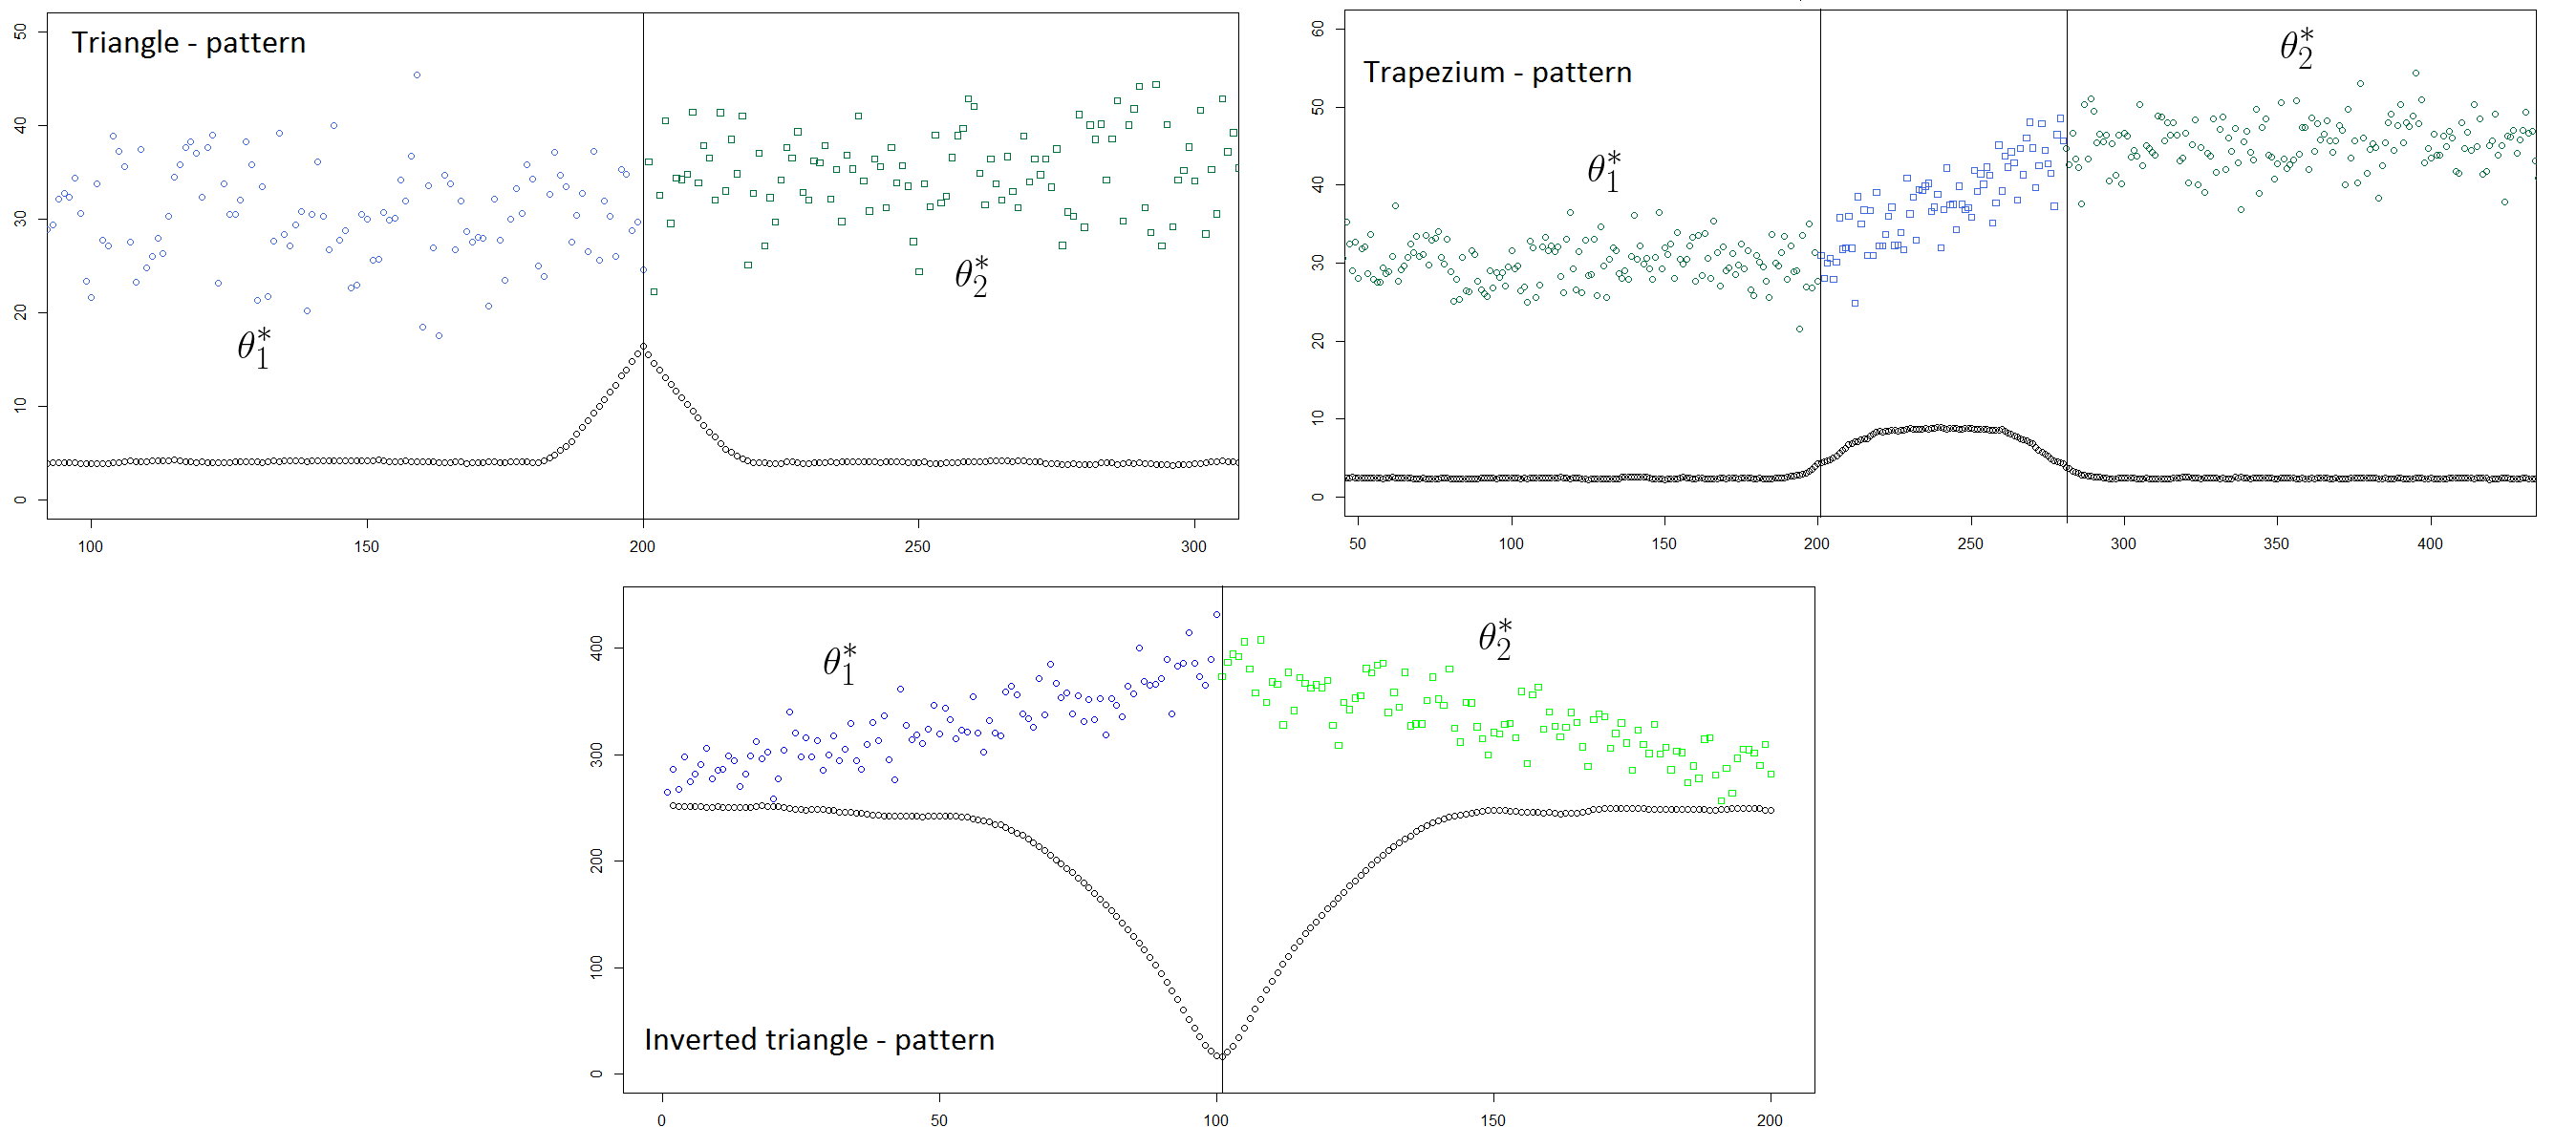
\includegraphics[width=0.9\textwidth, height=0.45\textwidth]{images/patterns-3.png}
    \caption{Type of change point and the geometry of change-point pattern}
    \label{fig:patterns}
\end{figure}

Any procedure of a change point detection requires information about the nature of the data observed after a structural break. The time of information aggregation is referred to as \textit{detection delay}. The proposed algorithm provides optimal \textit{detection delay} in the class of similar methods. The optimality is achieved by introduction of \textit{multiscale} approach. The technique is popular, e.g. \citet{multiscaleCP1}, \citet{SpokoinyCP} and allows analysis of the data using different scales simultaneously. The procedure proposed below computes the test statistics in rolling windows of different sizes and controls change-point pattern at each level. The greater number of scales at which a change-point pattern is detected, the more sure algorithm is, that there is a change point. 

Under some assumptions on the frequency of change points provided in Section~\ref{sec:theory}, the methods is applied to the \textit{multiple} change point problem. The survey on existing models can be found in \citet{chib98estimation}.
The last, but not at all the least feature of the proposed algorithm is that critical values for test statistic are computed in a data-driven way. The idea is to use the multiplier bootstrap procedure \citet{ChernozukovBoot}. The work of \citet{SpokoinyBoot}shows that it can be used for the construction of confides intervals even in case of a misspecified parametric model. Despite the fact, that theoretical properties of data-driven critical values are beyond the scope of this paper, the procedure of computation is presented in Algorithm~\ref{alg:bootstrap}.

The paper is organized as follows. Section~\ref{sec:procedure} presents the description of the algorithm. Theoretical properties of the procedure are discussed in Section~\ref{sec:theory}. Section~\ref{sec:experiments} compares the new algorithm with existing methods using simulated data sets. It also illustrates the performance of the method on a real data set. 

%To make the algorithm adaptive to change point of different sizes we introduce a . The LRT statistics is computed in rolling windows of different lengths. The approach and its modifications are quite popular in change point detection and for example is exploited in \citet{multiscaleCP1}, \citet{SpokoinyCP} and \citet{MultiscaleCP2}. The procedure relies on concept of multiscality is, for example, .Non-zero . It is referred to as The proof is based on novel algorithm of change point detection, that is described in the Section~\ref{sec:algorithm}.  an extension of \citet{LRTWilks} results to the finite-sample case. It shows that the behaviour of a fine sample is also $\chi^2$-like appropriate for multiple change point detection, e.g. \citet{multiscaleCP1}, \citet{chib1998estimation}. We assume change points \textcolor{red}{not to be very close to each other} and use \textit{multiscale} approach.  The similar idea of multiple testing for change \citet{SpokoinyCP} Thus, the introduction of \textit{multiscale} approach allows algorithm to be used for multiple Asumming that structural breaks are reasonably rare  frequency of the breaks %Nevertheless, it can be easily extended to retrospective frame work. The extension is presented in Section \ref{retrospective}.

%$Y_{i} \backsim \P_1$ if  and $Y_t \backsim \P_2$. 

%Let  $\mathbb{Y} = (Y_1, Y_2,..., Y_{\tau}, Y_{\tau + 1}...)$ be observed data. The goal is to detect a moment $\tau$ at which statistical properties of observed data change 

%Underlying assumption is that the structure of $\mathbb{Y}$ is homogeneous. It means that each $Y_i$ possess similar statistical properties. If the baseline assumption is wrong and the structure is non-homogeneous

%and $\mathbb{Y}$ is governed by some (presumably unknown) probability law $\P_1$.


%A change point is supposed to be detected if the hypothesis of homogeneity is rejected, in other words, there exists a moment $\tau$, $1 \leq \tau \leq N$, s.t. $(Y_1,..., Y_{\tau-1}) \backsim \P_1$ and $(Y_{\tau},..., Y_{N}) \backsim \P_2$, where $\P_2$ is not known as well. The moment $\tau$ is called a change-point. The goal is to find $\tau$ as precise as possible and minimise the number of false alarms and missed cases at the same time.
%